% \chapter{Proposed System}
% \section{Overview}
% The project is the development of  E Lib that aims to improve the efficiency and accuracy of the library management process. The software will be used by the library staff and admin to manage books, users, borrowing, returning, notifications, and generate reports and analytics. The objectives of the project are to automate and streamline the library management process, reduce human error, and improve the overall user experience. The project scope includes the development of the software, testing, and implementation.

\section{Functional Requirements}

\renewcommand{\arraystretch}{2}
\noindent
\begin{center}
\begin{tabular}{ | >{\bfseries}m{5em} | m{10cm} |  } 
  \hline
  ID & 3.2.1\\ 
  \hline
  Name & User and Administration \\ 
  \hline
  Description & 
  \begin{itemize}
      \item The system should allow the super admin to create and manage teacher and admin accounts through institutional mails.
      \item Teachers can update their account information.
      \item Allow password resets for all accounts.

  \end{itemize} \\
  \hline
  
  Priority & High\\
  \hline 
  Reference & \\
  \hline
\end{tabular}
\end{center}

\vspace{0.5cm}

\begin{center}
  \begin{tabular}{ | >{\bfseries}m{5em} | m{10cm} |  } 
    \hline
    ID & 3.2.2\\  
    \hline
    Name & Navbar \\  
    \hline
    Description & 
    \begin{itemize}
        \item Visualize University logo along with the department name
        \item Include quick links to pages, such as, Homepage, About, Admission, Teachers and Staff, Students Corner, Research, Academics, Events, Facilities and Alumni.
        \item Include quick links to login, logout pages
        \item Necessary quick links for admin
    \end{itemize} \\ 
    \hline
    Priority & High\\
    \hline 
    Reference & \\
    \hline
  \end{tabular}
  \end{center}

\begin{center}
\begin{tabular}{ | >{\bfseries}m{5em} | m{10cm} |  } 
  \hline
  ID & 3.2.3\\  
  \hline
  Name & Homepage \\  
  \hline
  Description & 
  \begin{itemize}
      \item Should display a welcome message.
      \item Show the department’s mission and vision.
      \item Provide announcements and news updates.
      \item Display upcoming events.
  \end{itemize} \\ 
  \hline
  Priority & High\\
  \hline 
  Reference & \\
  \hline
\end{tabular}
\end{center}

\vspace{0.5cm}


\begin{center}
\begin{tabular}{ | >{\bfseries}m{5em} | m{10cm} |  } 
  \hline
  ID & 3.2.4\\  
  \hline
  Name & About Us \\  
  \hline
  Description & 
  \begin{itemize}
      \item Provide an overview of the department.
      \item Include a message from the Head of the Department.
      \item Showcase department history and achievements.
      \item Show contact information and location on a map.
  \end{itemize} \\ 
  \hline
  Priority & Medium\\
  \hline 
  Reference & \\
  \hline
\end{tabular}
\end{center}

\vspace{0.5cm}


\begin{center}
\begin{tabular}{ | >{\bfseries}m{5em} | m{10cm} |  } 
  \hline
  ID & 3.2.5\\  
  \hline
  Name & Academics \\  
  \hline
  Description & 
  \begin{itemize}
      \item Provide information about undergraduate, postgraduate, and PhD programs.
      \item Display course structures, syllabi, and credit details.
      \item Include class schedules and timetables.
      \item Provide an academic calendar with important dates.
  \end{itemize} \\ 
  \hline
  Priority & High\\
  \hline 
  Reference & \\
  \hline
\end{tabular}
\end{center}

\vspace{0.5cm}


\begin{center}
\begin{tabular}{ | >{\bfseries}m{5em} | m{10cm} |  } 
  \hline
  ID & 3.2.6\\  
  \hline
  Name & Faculty and Staff \\  
  \hline
  Description & 
  \begin{itemize}
      \item Maintain a faculty directory with names, designations, and research backgrounds.
      \item Provide links to faculty members' LinkedIn and Google Scholar profiles.
      \item Display faculty and staff details, office room numbers, and office hours.
  \end{itemize} \\ 
  \hline
  Priority & High\\
  \hline 
  Reference & \\
  \hline
\end{tabular}
\end{center}

\vspace{0.5cm}


\begin{center}
\begin{tabular}{ | >{\bfseries}m{5em} | m{10cm} |  } 
  \hline
  ID & 3.2.7\\  
  \hline
  Name & Research and Innovation \\  
  \hline
  Description & 
  \begin{itemize}
      \item Provide information on research areas and groups.
      \item Show research publications and ongoing projects.
      \item Display collaboration opportunities and funding options.
  \end{itemize} \\ 
  \hline
  Priority & Medium\\
  \hline 
  Reference & \\
  \hline
\end{tabular}
\end{center}

\vspace{0.5cm}


\begin{center}
\begin{tabular}{ | >{\bfseries}m{5em} | m{10cm} |  } 
  \hline
  ID & 3.2.8\\  
  \hline
  Name & Admissions \\  
  \hline
  Description & 
  \begin{itemize}
      \item Provide admission criteria and process details.
      \item Allow applicants to download and submit application forms.
      \item Display scholarship and financial aid information.
      \item Provide an FAQ section related to admissions.
  \end{itemize} \\  
  \hline
  Priority & High\\
  \hline 
  Reference & \\
  \hline
\end{tabular}
\end{center}

\vspace{0.5cm}


\begin{center}
\begin{tabular}{ | >{\bfseries}m{5em} | m{10cm} |  } 
  \hline
  ID & 3.2.9\\  
  \hline
  Name & Student Corner \\  
  \hline
  Description & 
  \begin{itemize}
      \item Display information on student clubs and their activities, and other organizations.
      \item Highlight student achievements.
      \item Provide access to academic resources such as lecture notes and past question papers.
  \end{itemize} \\ 
  \hline
  Priority & Medium\\
  \hline 
  Reference & \\
  \hline
\end{tabular}
\end{center}

\vspace{0.5cm}

\begin{center}
  \begin{tabular}{ | >{\bfseries}m{5em} | m{10cm} |  } 
    \hline
    ID & 3.2.10\\  
    \hline
    Name & Notices and Circulars \\  
    \hline
    Description & 
    \begin{itemize}
        \item Allow admins to publish official announcements.
        \item Provide department policies, rules, and regulations.
        \item Display exam schedules, results, and other academic notices.
    \end{itemize} \\ 
    \hline
    Priority & High\\
    \hline 
    Reference & \\
    \hline
    
  \end{tabular}
\end{center}

\vspace{0.5cm}

\begin{center}
\begin{tabular}{ | >{\bfseries}m{5em} | m{10cm} |  } 
  \hline
  ID & 3.2.11\\  
  \hline
  Name & Events and Conferences \\  
  \hline
  Description & 
  \begin{itemize}
      \item Display information on upcoming workshops and seminars.
      \item Provide details on hackathons and coding competitions.
      \item Show details on departmental events such as covocations, parties, and picnics etc
      \item Provide event participation details and allow registration
  \end{itemize} \\ 
  \hline
  Priority & Medium\\
  \hline 
  Reference & \\
  \hline
\end{tabular}
\end{center}

\vspace{0.5cm}


\begin{center}
\begin{tabular}{ | >{\bfseries}m{5em} | m{10cm} |  } 
  \hline
  ID & 3.2.12\\  
  \hline
  Name & Alumni \\  
  \hline
  Description & 
  \begin{itemize}
      \item Showcase alumni success stories.
      \item Provide information on alumni networks and events.
  \end{itemize} \\ 
  \hline
  Priority & Low\\
  \hline 
  Reference & \\
  \hline
\end{tabular}
\end{center}

\vspace{0.5cm}

\begin{center}
\begin{tabular}{ | >{\bfseries}m{5em} | m{10cm} |  } 
  \hline
  ID & 3.2.13\\  
  \hline
  Name & Facilities \\  
  \hline
  Description & 
  \begin{itemize}
      \item Provide information on departmental facilities such as labs, libraries, and auditoriums.
  \end{itemize} \\ 
  \hline
  Priority & Medium\\
  \hline 
  Reference & \\
  \hline
\end{tabular}
\end{center}

\vspace{0.5cm}

\begin{center}
\begin{tabular}{ | >{\bfseries}m{5em} | m{10cm} |  } 
  \hline
  ID & 3.2.14\\  
  \hline
  Name & AI Assistant \\  
  \hline
  Description & 
  \begin{itemize}
      \item Implement an AI assistant to promptly answer frequently asked questions.
      \item Provide information on admission, courses, faculty, and events.
      \item Allow users to ask questions, and get answers in both Bengali and English.
  \end{itemize} \\ 
  \hline
  Priority & Medium\\
  \hline 
  Reference & \\
  \hline
  
\end{tabular}
\end{center}

\section{Nonfunctional Requirements}
\begin{enumerate}
    \item Performance Requirements
    \begin{itemize}
        \item The system should respond to user requests within \textbf{2 seconds} under normal load.
        \item It should support at least \textbf{1000 concurrent users} without performance degradation.
        \item Database queries should be optimized to execute within \textbf{500 milliseconds} on average.
        \item The system should be able to handle a \textbf{10,000-record dataset} efficiently.
    \end{itemize}

    \item Security Requirements
    \begin{itemize}
        \item User authentication should be enforced using \textbf{OAuth 2.0 or JWT-based authentication}.
        \item Institutional email verification should be required for teacher and admin accounts.
        \item Passwords should be \textbf{hashed and stored securely} using bcrypt or Argon2.
        \item The system should prevent \textbf{SQL injection, cross-site scripting (XSS), and cross-site request forgery (CSRF)}.
        \item Role-based access control (RBAC) should be implemented to restrict access to different sections of the system.
    \end{itemize}

    \item Usability Requirements
    \begin{itemize}
        \item The user interface should be \textbf{intuitive and accessible} to users of different technical backgrounds.
        \item The system should follow \textbf{WCAG 2.1 Level AA} accessibility standards.
        \item Mobile responsiveness should be ensured across devices with different screen sizes.
        \item The system should support \textbf{Bengali and English languages}.
    \end{itemize}

    \item Availability Requirements
    \begin{itemize}
        \item The system should have \textbf{99.5\% uptime} except for planned maintenance.
        \item In case of a failure, the system should be \textbf{recoverable within 30 minutes}.
        \item Automated database backups should be scheduled \textbf{daily} and retained for at least \textbf{30 days}.
    \end{itemize}

    \item Maintainability and Scalability
    \begin{itemize}
        \item The system should follow a \textbf{modular architecture} for easy maintenance and updates.
        \item The backend should be designed using \textbf{RESTful API principles}, and \textbf{Software Design Best Practices and Patterns}.
        \item The system should be \textbf{horizontally scalable} to accommodate an increase in users.
        \item The system should be \textbf{vertically scalable} to accommodate an increase in data (such as, resources) volume.
        \item Logging and monitoring should be implemented using \textbf{ELK stack or Prometheus}.
    \end{itemize}

    \item Data Integrity and Consistency
    \begin{itemize}
        \item The database should maintain \textbf{ACID compliance} for transactions.
        \item The system should ensure that \textbf{no duplicate user accounts} are created.
        \item All updates to the database should follow \textbf{proper validation and constraints}.
    \end{itemize}

    \item Compatibility Requirements
    \begin{itemize}
        \item The frontend should be \textbf{compatible with modern browsers} (Chrome, Firefox, Edge, Safari).
        \item The backend should be deployable on \textbf{Linux-based cloud servers}.
        \item The database should support either \textbf{SQL-based relational models (PostgreSQL/MySQL/SQLite)} or \textbf{no SQL models (MongoDB/Redis)}.
    \end{itemize}

    \item Logging and Monitoring
    \begin{itemize}
        \item All system events should be \textbf{logged with timestamps and user activity}.
        \item Error logs should be stored and categorized based on severity.
        \item A monitoring dashboard should be available for \textbf{system health checks}.
    \end{itemize}

    \item Disaster Recovery and Backup
    \begin{itemize}
        \item The system should have a \textbf{disaster recovery plan} to restore services quickly.
        \item Backups should be \textbf{stored in a separate location} to avoid single-point failure.
        \item Regular \textbf{testing of backup restoration} should be performed.
    \end{itemize}
\end{enumerate}
% \section{System Model}
% \subsection{Scenarios}

% \subsubsection{Create new user account}

% \begin{itemize}
%     \item Admin can create new user account.
%     \item Admin gives different information for the account.
%     \item Only Admin can access create new user section.
% \end{itemize}

% \subsubsection{Member Maintenance}

% \begin{itemize}
%     \item Librarian and staffs who have user account maintain the member of the library.
%     \item User can update ,delete the information of the member.
%     \item Book lending facilities for the member also maintain by the users.
% \end{itemize}

% \subsubsection{Book Management}

% \begin{itemize}
%     \item User can add books according to their section,subsection and categories.
%     \item User can filter the books on basis of category.
%     \item user can update quantity or availability of the books.
% \end{itemize}

% \subsubsection{Book Transaction}

% \begin{itemize}
%     \item Users handle the book transaction section.
%     \item Users update the information like status,borrowing date,returning date etc related to each transaction
% \end{itemize}

% \subsubsection{Book Return}
% \begin{itemize}
%     \item Users make sure that the book must be returned in the selected date.
%     \item After returning book users update the information. 
% \end{itemize}



% \subsection{Use cases}
% \begin{center}

% Create account
\begin{tabular}{ | m{7em} | m{9cm}|} 
  \hline
  Name & Create new account\\ 
  \hline    
  Actor & Admin \\ 
  \hline
  Flow of events & 
    System Admin will create a new account for other librarian and stuff. With the account created , Librarian will have the access to the software. \\
  \hline
  
  Entry Condition & Admin will give information about the new account taken from the library stuff. \\
  \hline
  Exit Condition & The app will create the account, store it in the local database and display it \\
  \hline

\end{tabular}

\vspace{1cm}

\begin{tabular}{ | m{7em} | m{9cm}|} 
  \hline
  Name & Login\\ 
  \hline    
  Actor & Admin , Librarian \\ 
  \hline
  Flow of events & 
    1. User enters email and password
    \newline
    2. User clicks on "Log In" button\\
  \hline
  
   Entry Condition & The user is not logged in and has a registered account  \\
  \hline
  Exit Condition & The user is logged in and taken to the home screen \\
  \hline

\end{tabular}

\vspace{1cm}

\begin{tabular}{ | m{7em} | m{9cm}|} 
  \hline
  Name & Logout\\ 
  \hline    
  Actor &  Admin , Librarian \\ 
  \hline
  Flow of events & 
 User clicks on "Log Out" button \\
  \hline
  
   Entry Condition & The user is logged in \\
  \hline
  Exit Condition & The user is logged out and taken to the login screen \\
  \hline

\end{tabular}

\vspace{1cm}

\begin{tabular}{ | m{7em} | m{9cm}|} 
  \hline
  Name & Update Profile\\ 
  \hline    
  Actor & Admin , Librarian \\ 
  \hline
  Flow of events & 

    1. User selects "Edit Profile" option 
    \newline
    2. User makes desired changes to their profile information
    \newline
    3. User clicks on "Save" button \\
    
  \hline
 
   Entry Condition & The user is logged in .\\
  \hline
  Exit Condition & User's profile information is updated and saved.\\
  \hline

\end{tabular}

\vspace{1cm}

\begin{tabular}{ | m{7em} | m{9cm}|} 
  \hline
  Name & Maintain Book Records\\ 
  \hline    
  Actor & Admin , Librarian \\ 
  \hline
  Flow of events & 

   1. Add Book: Admin/Librarian adds a new book to the library's collection by filling out the book's information in the system.
       \newline
   2.Remove Book: Admin/Librarian removes a book from the library's collection by deleting the book's record from the system.
       \newline
    3. Update Book Info: Admin/Librarian updates a book's information in the system, such as the title, author, or publisher.
        \newline
    4. Add Category/Sub Category: Admin/Librarian adds a new book category to the system. \\
  \hline
  
   Entry Condition & Admin/Librarian is logged in \\
  \hline
  Exit Condition & The book records are updated in the system and the Admin/Librarian can continue to manage the library's book collection.
 \\
  \hline

\end{tabular}

\vspace{1cm}

\begin{tabular}{ | m{7em} | m{9cm}|} 
  \hline
  Name & Issue / Return Book\\ 
  \hline    
  Actor & Admin , Librarian, Member \\ 
  \hline
  Flow of events & 

  1. The librarian or admin searches for the book in the system
  \newline
   2. If the book is available, the librarian or admin processes the borrowing or returning request
     \newline
3.  The system updates the book status accordingly
  \newline
4.  The librarian or admin provides the book to the member (in the case of borrowing) or receives the book from the member (in the case of returning) \\
  \hline
     Entry Condition &
    1. A member requests to borrow or return a book
    \newline
    2.The librarian or admin is logged in and has access to the system\\
  \hline
  Exit Condition & The book is successfully borrowed or returned. \\
  \hline

\end{tabular}

\vspace{1cm}

\begin{tabular}{ | m{7em} | m{9cm}|} 
  \hline
   Name & Maintain Members\\ 
  \hline    
  Actor & Admin , Librarian \\ 
  \hline
  Flow of events & 

    Admin/Librarian adds, removes or updates member information \\
  \hline
  
   Entry Condition & Admin/Librarian is logged in and authorized to maintain member records \\
  \hline
  Exit Condition & Member record is added, removed or updated in the system, and the Admin/Librarian is notified of the action. \\
  \hline

\end{tabular}


\vspace{1cm}

\end{center}


% \subsection{Use case diagram}
% \begin{figure}[H]
%     \centering
%     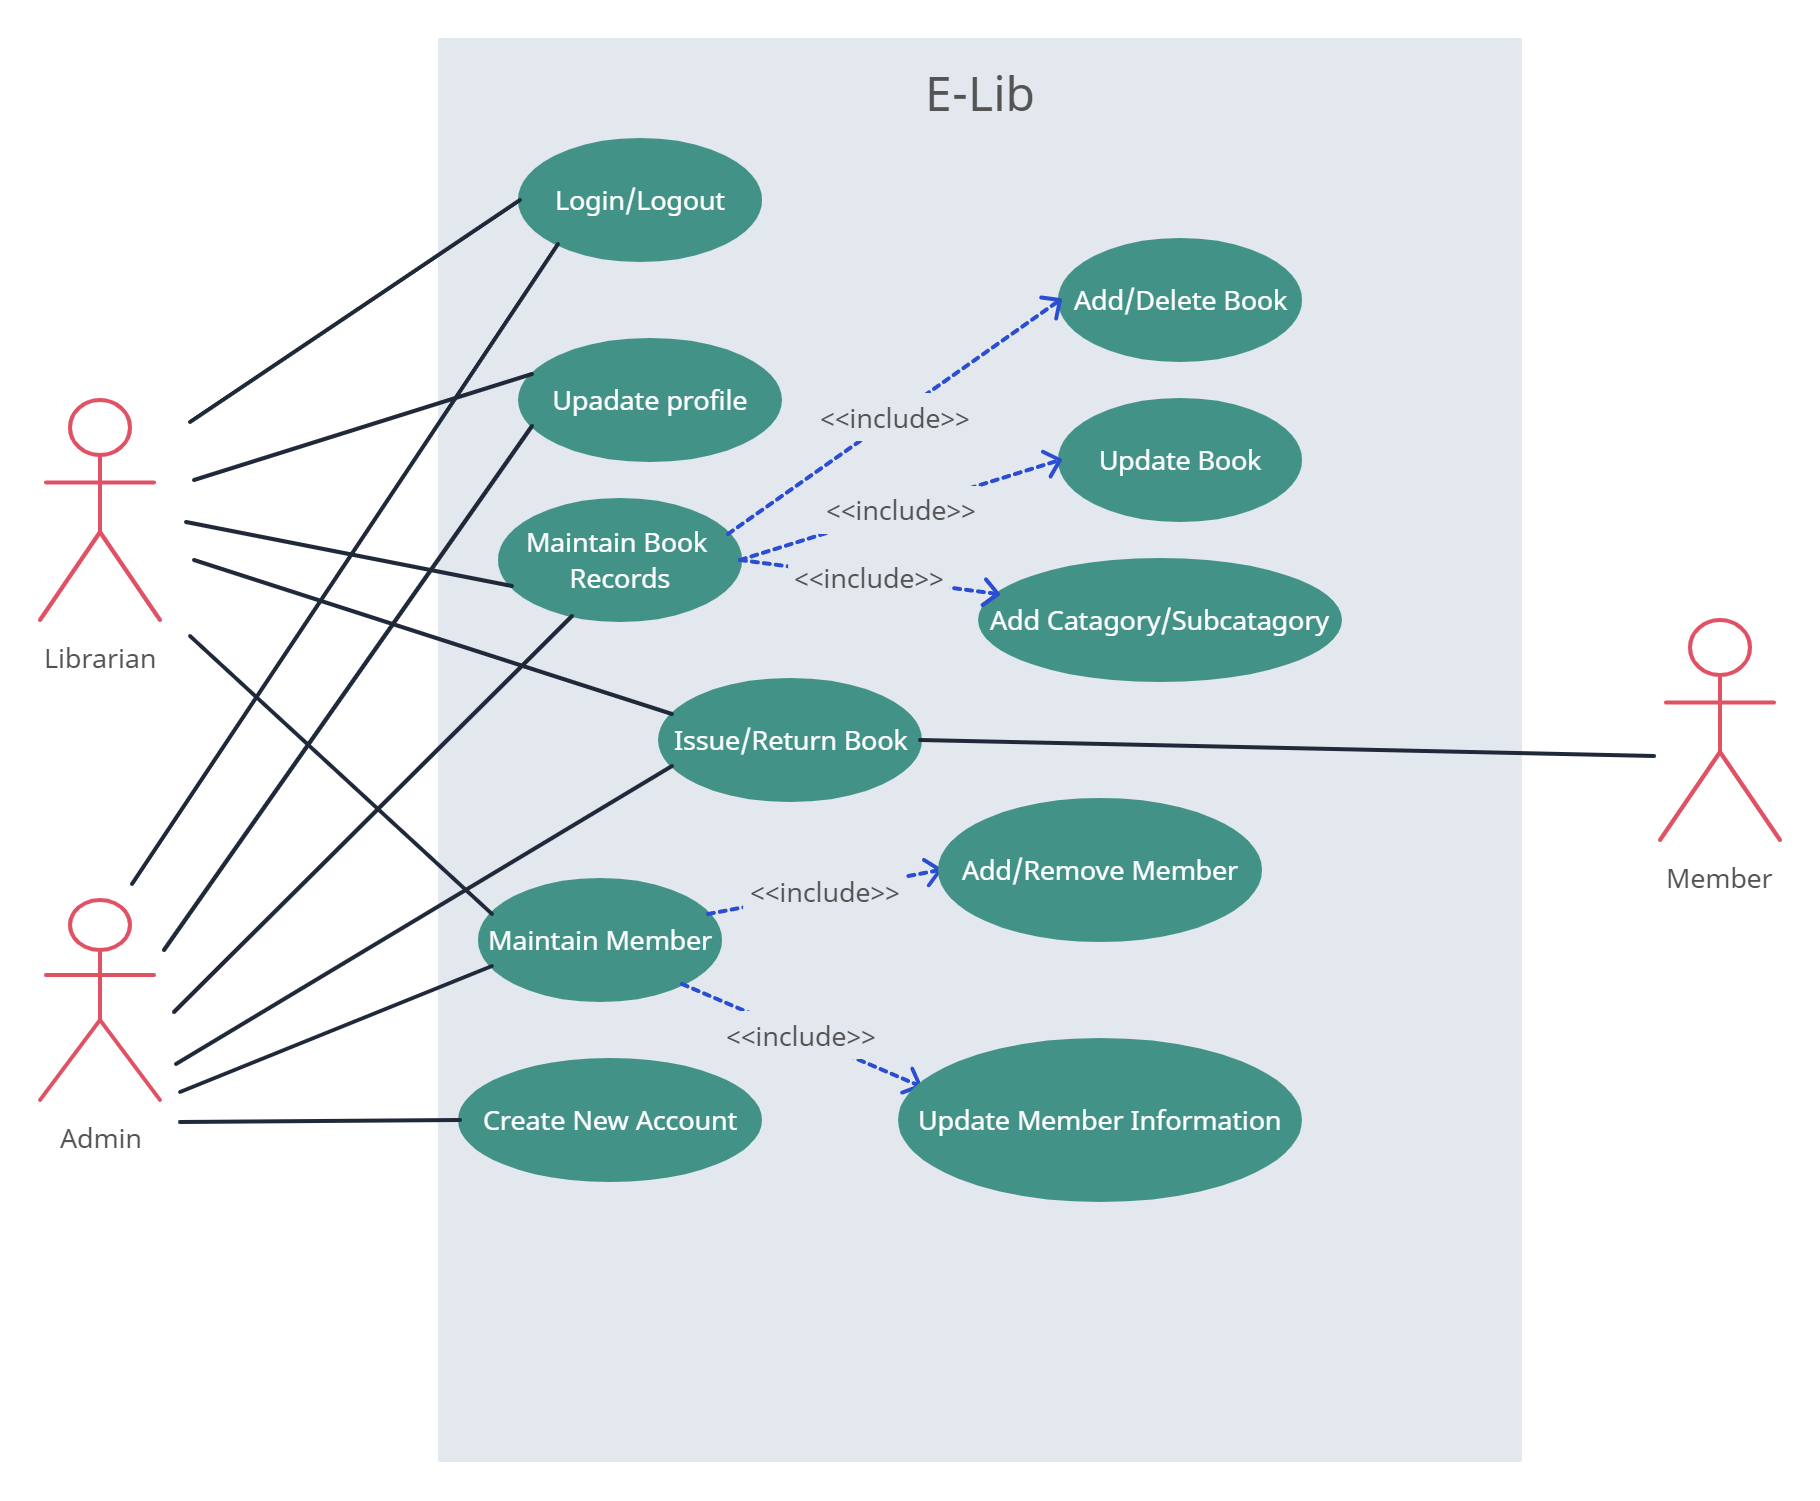
\includegraphics[scale = 0.27]{images/useCase.png}
%     \caption{Use Case Diagram}
%     \label{fig:use_case_diagram}
% \end{figure}

% \subsection{Dynamic model}
% \subsubsection{Sequence Model}
% \begin{figure}[H]
%     \centering
%     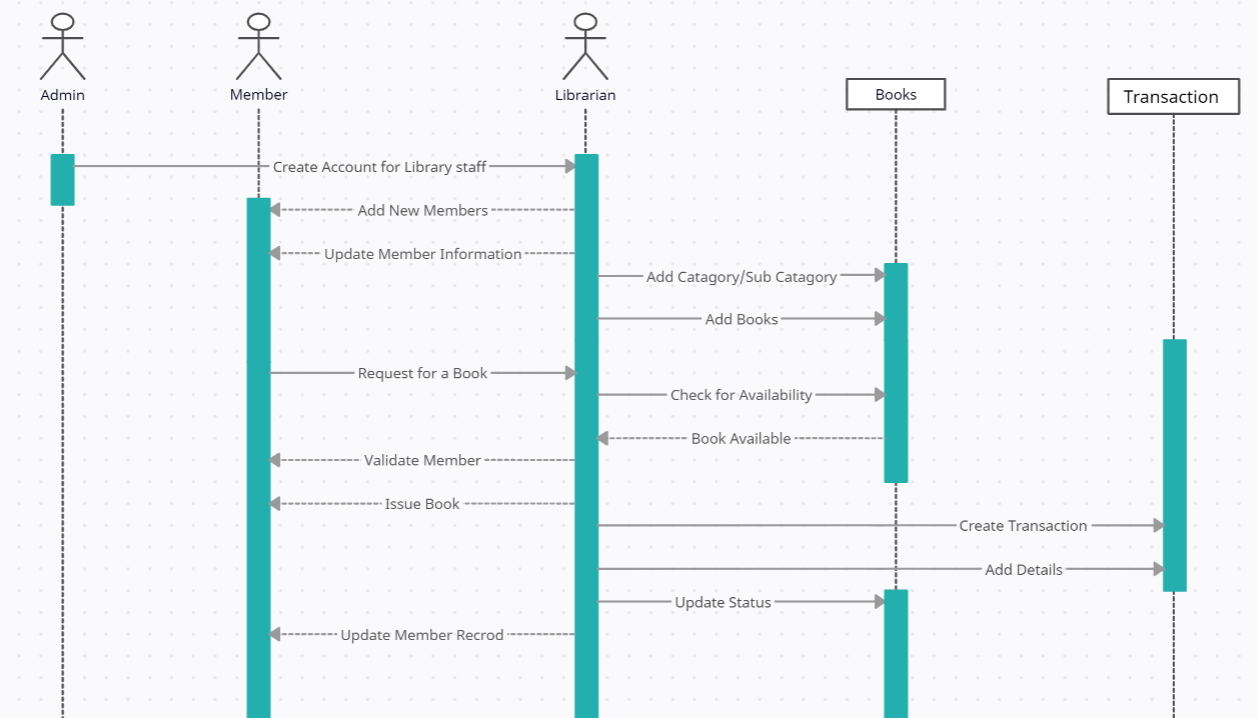
\includegraphics[width=\textwidth]{images/sequence.png}
%     \caption{Sequence Diagram}
%     \label{fig:sequence_diagram}
% \end{figure}

% \subsubsection{Statechart model}
% \begin{figure}[H]
%     \centering
%     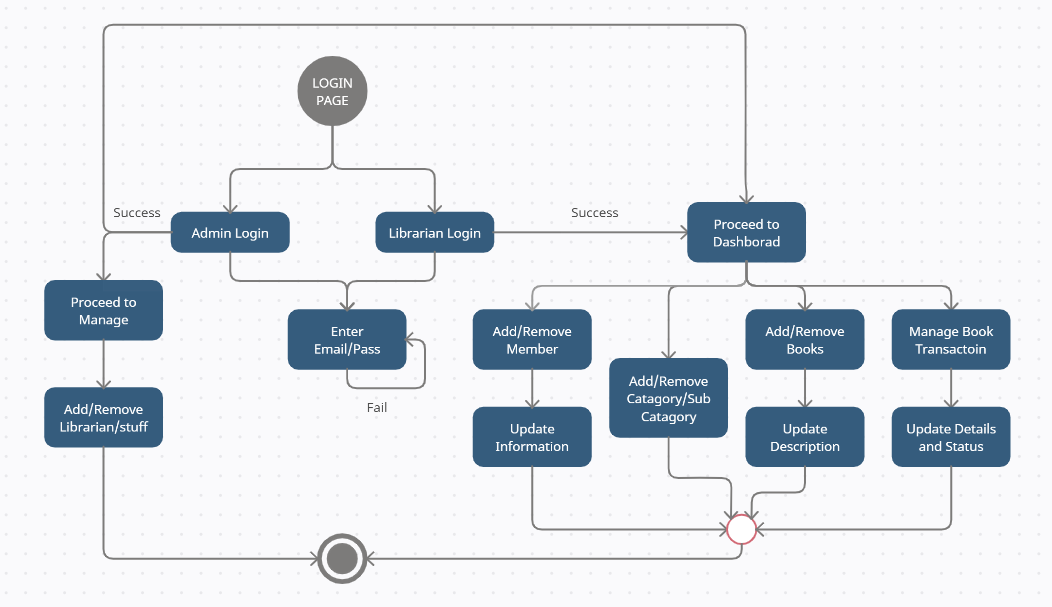
\includegraphics[width=\textwidth]{images/statechartr.png}
%     \caption{Statechart Diagram}
%     \label{fig:statechart_diagram}
% \end{figure}

% \subsection{Activity Diagram}
% \begin{figure}[H]
%     \centering
%     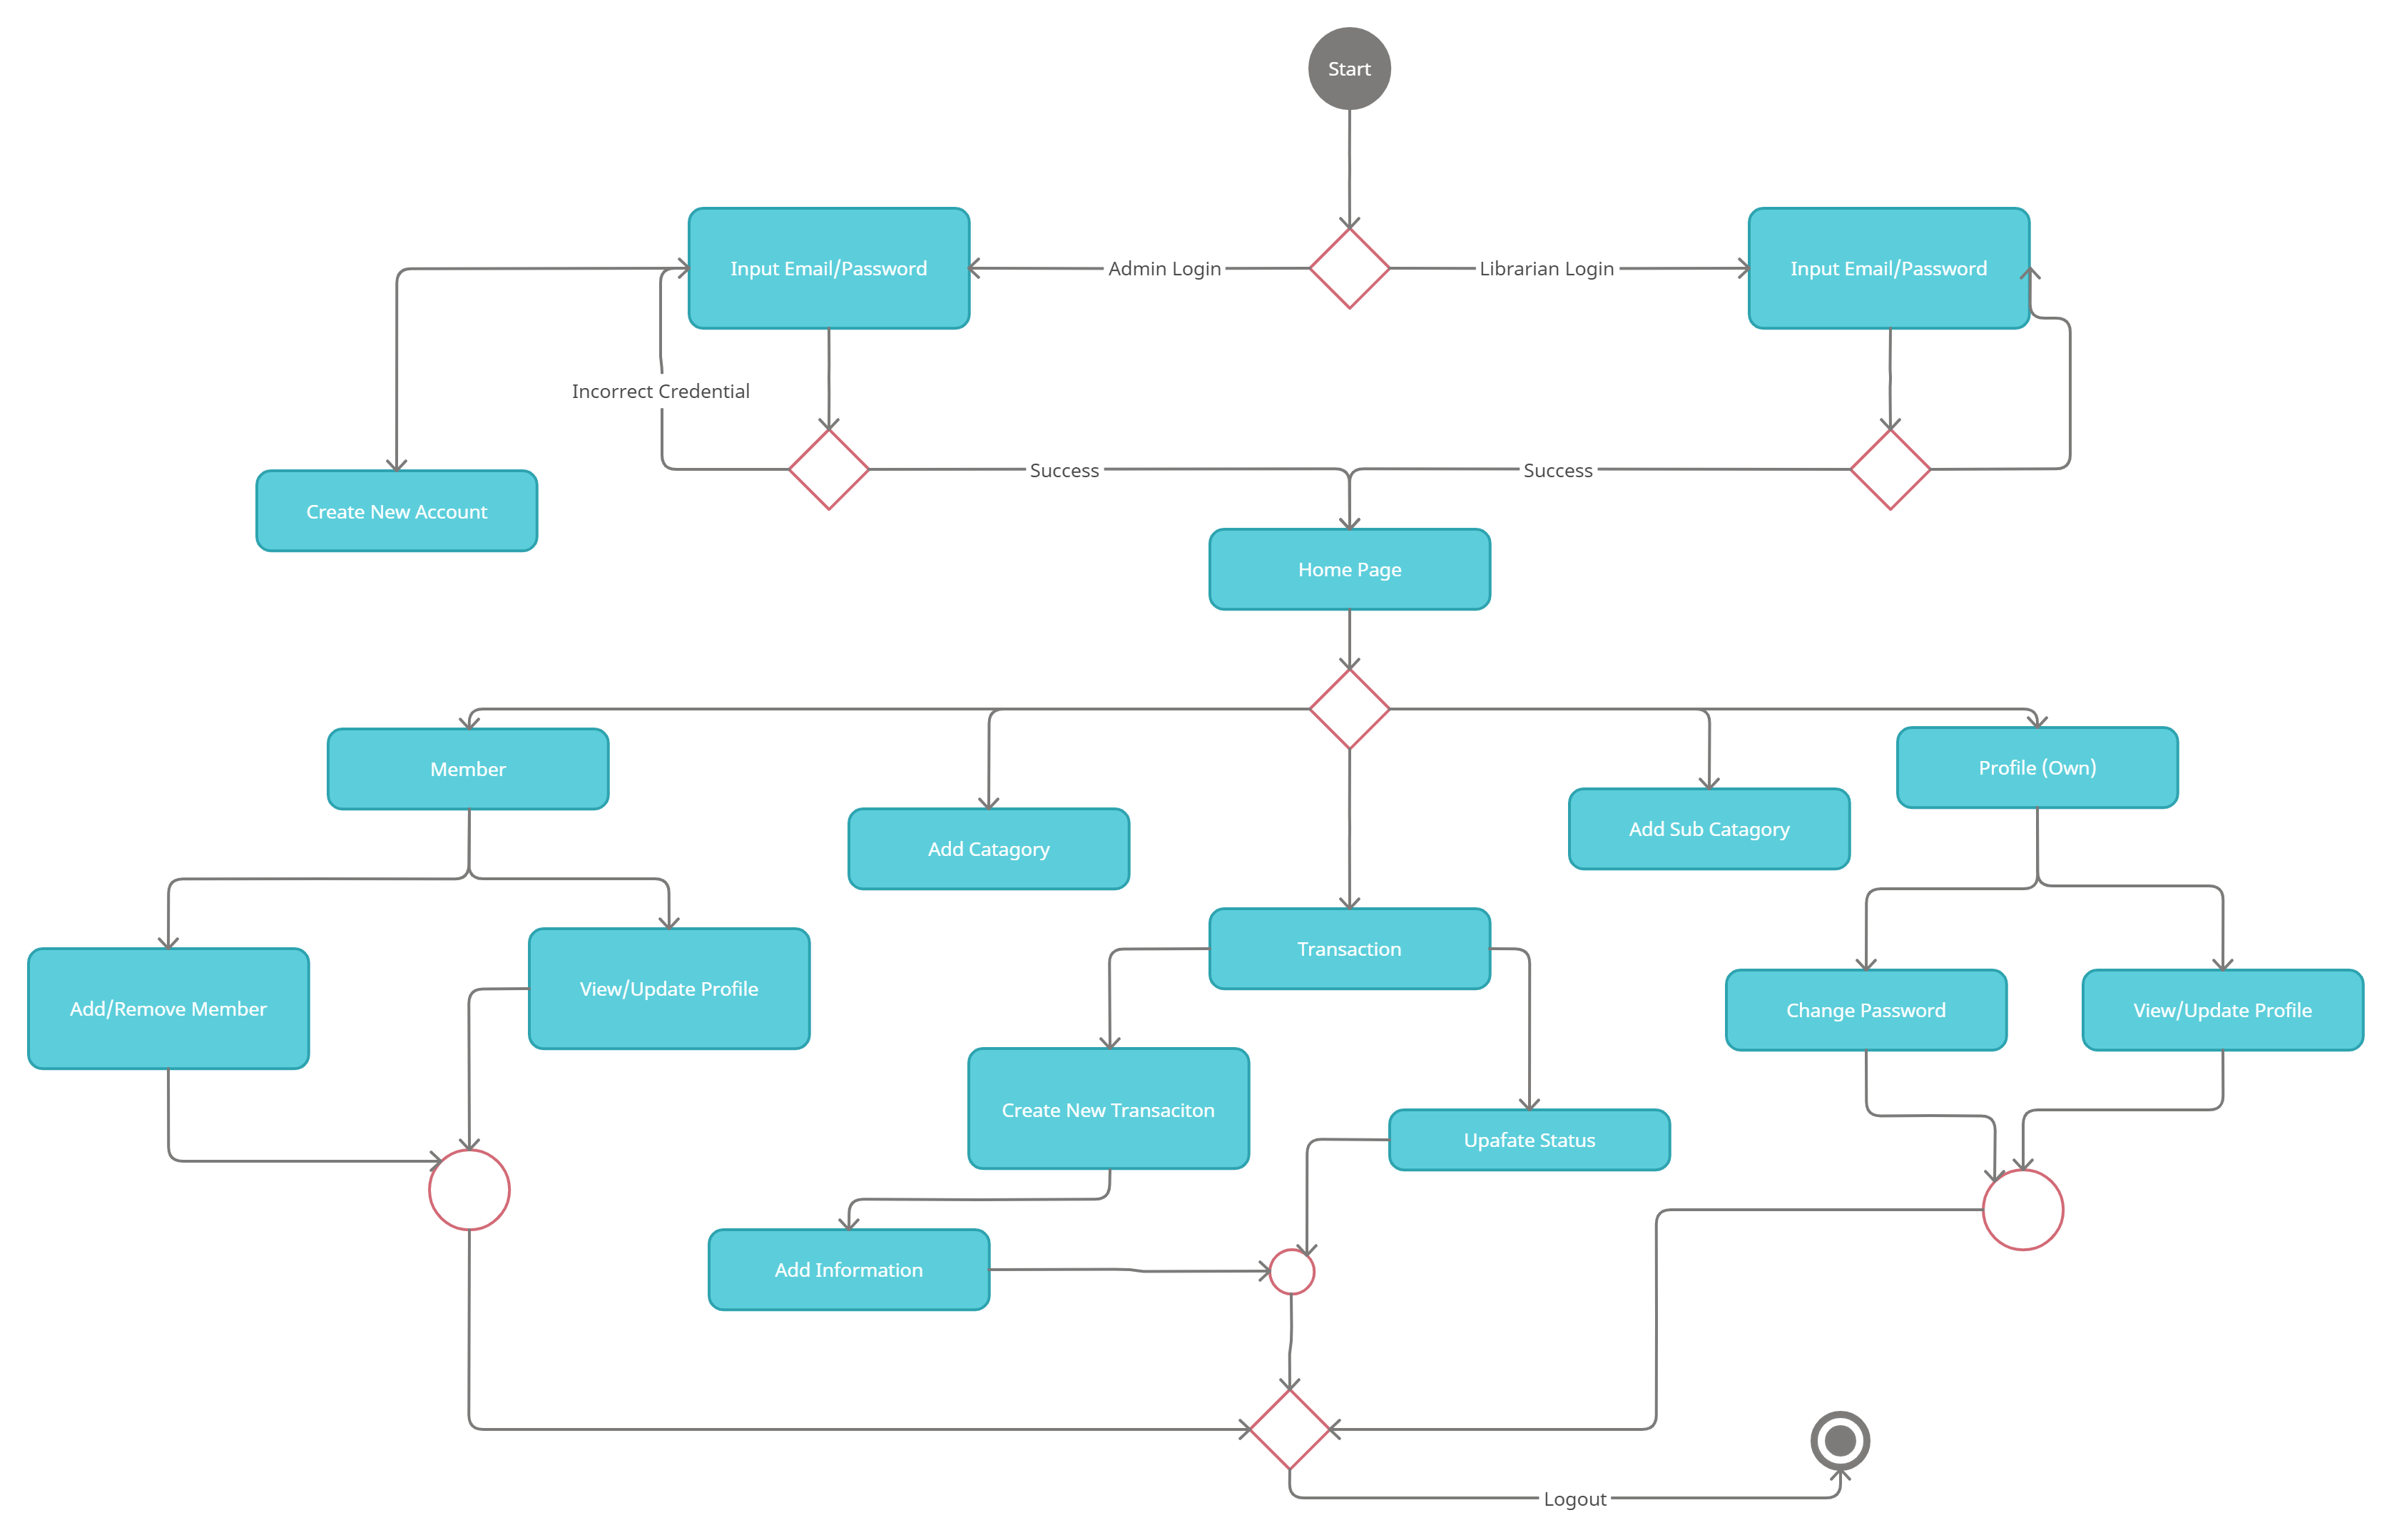
\includegraphics[width=\textwidth]{images/activity.png}
%     \caption{Activity Diagram}
%     \label{fig:activity_diagram}
% \end{figure}
% \newpage
% \subsection{User interface}

% \subsubsection{Home Page}
% The Home page shows statistics of all the options for the system which includes Home,Category,Sub Category,Books,Students,Borrowing Transaction,User etc. There will be a menu bar above, which will show the options.

% \subsubsection{Menu Bar}
% Admin can be able to access all of the sections of menu-bar.But Librarian and other staffs can't access user section part. In this specific section , new user for the software can be added

% \subsubsection{Categories}
% In this section the books will arrange according to their category.The description and the date from when the book has been added will be provided.Here will be the action part in which the users can update,remove or view the books.Here Users can add the books by filling up the information about the book and the searching option will 
% also available in this page.

% \subsubsection{Subcategories}
% It will be same as categories page.The main deference is it will provide the information more specific for the users.All the options which are available in the Categories page will also be available in this page.

% \subsubsection{Books}
% In this section books will be displayed with their category/subcategory,title,id added date ,status, action etc.Book searching option will be available in this section.User can add new book ,update the information ,remove and view the book.

% \subsubsection{Member}
% This section will provide the information of the library member.The information like name,ID,Added date will be available.Users can add or remove the member if they want.There will be update or view option for editing or viewing member's information.Searching option will also available.

% \subsubsection{Transaction}
% In this section users can add the information of borrowing and returning book.Users will keep the record of the members who will borrow or return the book with their name,id and the book name which will be transacted.

% \subsubsection{Create New Account}
% Admin can only access this section.Admin can add new account.Other users (Librarian,Stuffs) won't have the access to create new account.


% \subsubsection{Software Interface}
% The project is a web based application. Hence it will need a working web browser and windows OS. The app can be kept in the pc's memory and can be runned locally.

% \subsubsection{Hardware Interface}
% The app will need the keyboard/mouse to interfere with the user. 